% Generated by tex/build_swebok_structure.py from tex/chapters/ch01/03_ソフトウェア要求の基礎.tex
\subsubsection{ソフトウェア要求の分類}

要求は、すべてをひとまとめにすると扱いにくい。SWEBOKでは、ソフトウェア要求を大きく次のように整理する。

\begin{center}
\footnotesize
\par\smallskip\noindent\refstepcounter{table}\label{tab:ch01-02}\textbf{表 \thetable: 第01章 ソフトウェア要求 表02}\par\smallskip
\begin{tabular}{c}
ソフトウェア要求 \\
$\downarrow$ \\
ソフトウェア製品要求 \quad / \quad ソフトウェアプロジェクト要求 \\
$\downarrow$ \\
機能要求 \quad / \quad 非機能要求 \\
$\downarrow$ \\
技術制約 \quad / \quad サービス品質制約
\end{tabular}
\end{center}

\begin{figure}[htbp]
\centering
\IfFileExists{assets/generated_figures/ch01/fig-ch01-02.png}{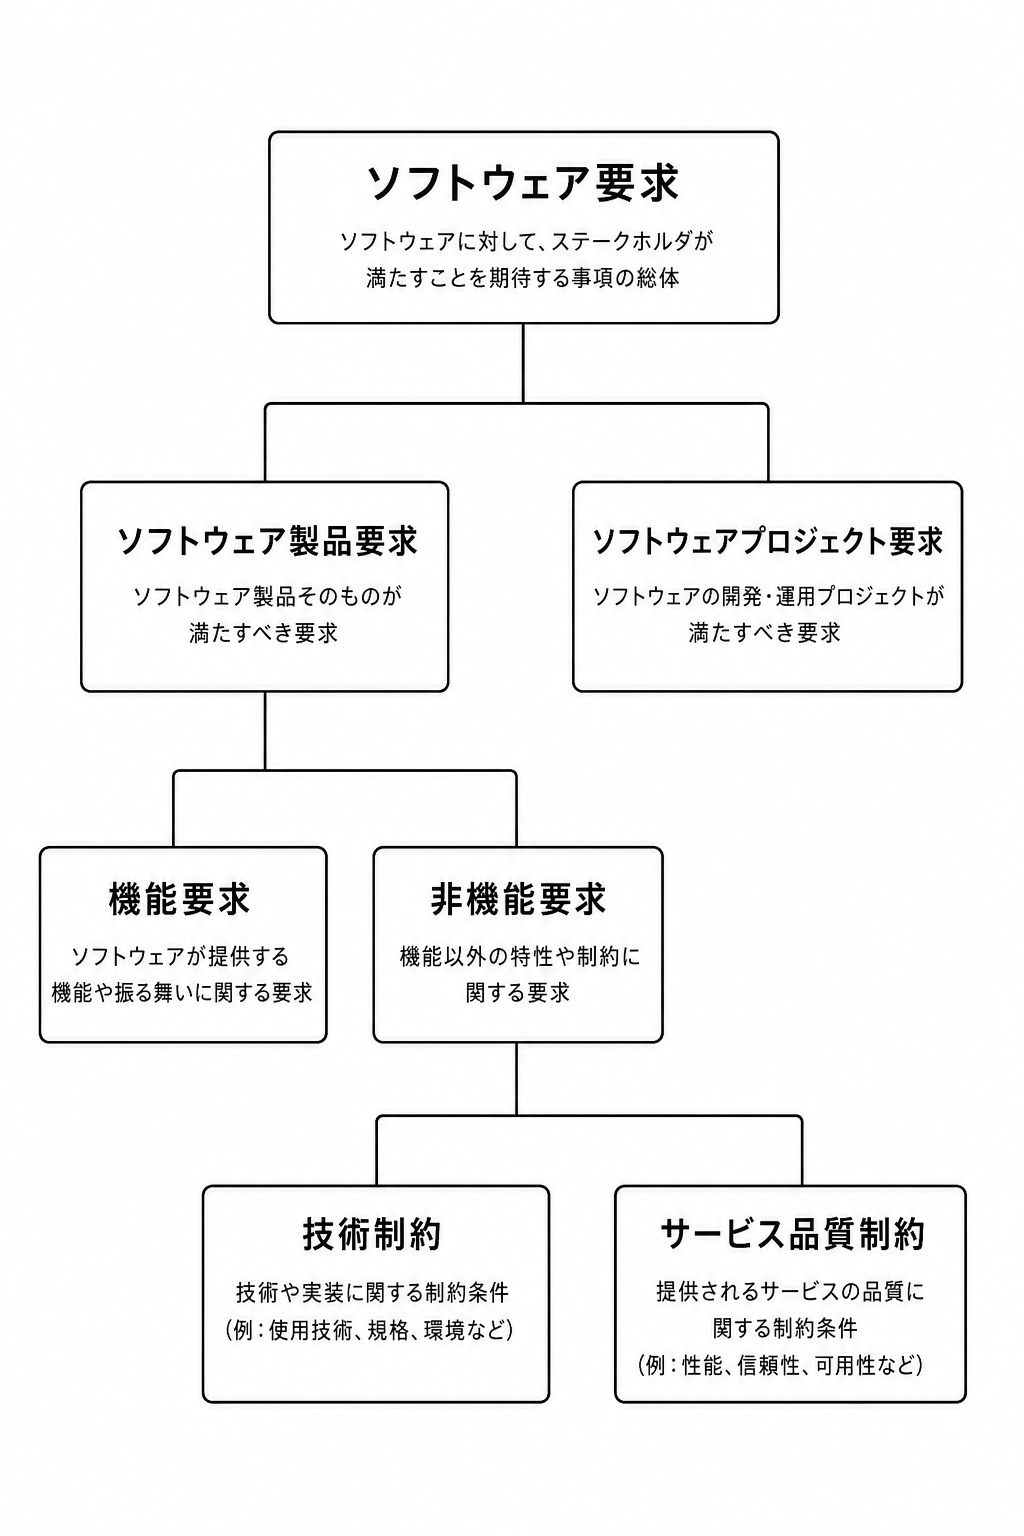
\includegraphics[width=0.96\linewidth]{assets/generated_figures/ch01/fig-ch01-02.png}}{\fbox{\parbox[c][48mm][c]{0.9\linewidth}{\centering 画像生成待ち\\要求分類の階層図}}}
\caption{要求分類の階層図}
\label{fig:ch01-02}
\end{figure}

分類の目的は、単に用語を覚えることではない。分類すると、要求の源泉、引き出し方、分析方法、仕様化の方法、確認すべき相手が見えやすくなる。
